% reset section counter
%\setcounter{section}{0}

%\metadata{lecture ID}{Your names}{date}
\metadata{13}{Justin Young and Josh Cho}{November 1, 2021}

\sec{The Neural Tangent Kernel (NTK) Approach}

In the previous sections, we studied non-convex optimization problems in which all local minima are global. Selecting the parameters of a deep neural network is another commonly encountered non-convex optimization problem, but it is unrealistic to expect that all local minima will also be global minima in this setting. Here we consider a particular objective for which we can identify particular regions of the input space in which all local minima are also global minima. We can show that this objective corresponds to certain types of deep neural networks, but this analysis remains limited. For further reading about this approach to studying neural network optimization, see \cite{liang2018adding} and \cite{du2019gradient}.

\tnotelong{Tengyu should  double check this later}

To be more formal, we take an appropriate parameter initialization $\theta^0$ such that in a neighborhood around it, which we denote by $B(\theta^0)$, the loss function is convex and its global minimum is attained. Figure \ref{lec13:fig:NTKapproach} depicts a function and region for which this condition holds. 

\begin{figure}[ht]
    \centering
    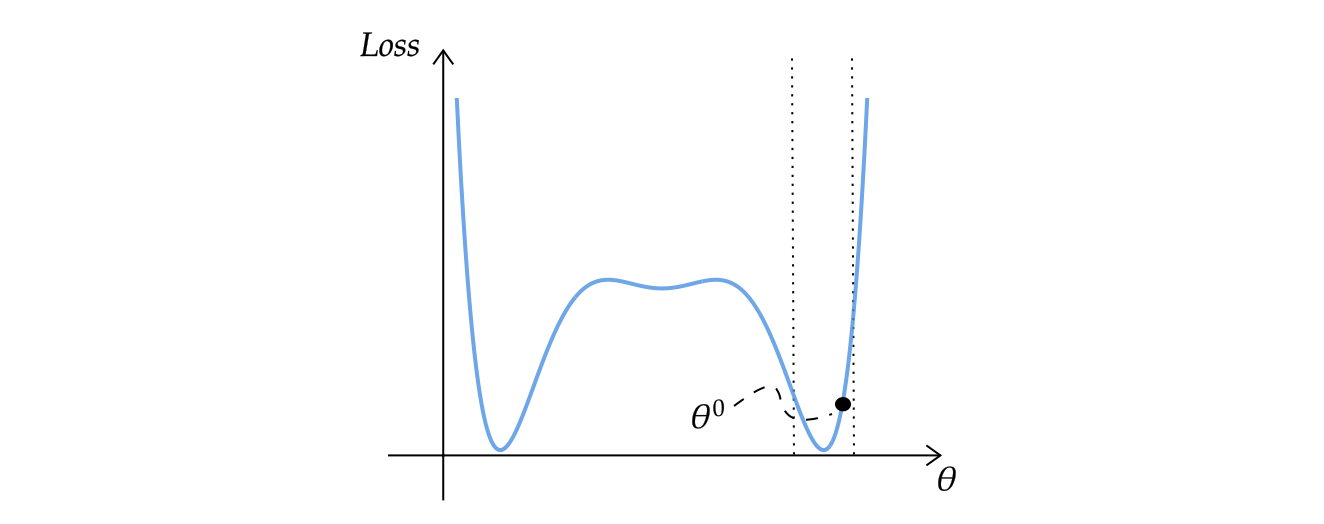
\includegraphics[scale=0.3]{figures/ntk_initialization.png}
    \caption{Training loss around an initialized $\theta^0$. The dotted lines indicate $B(\theta^0)$, a region where the loss is convex, and where a global minimum exists.}
    \label{lec13:fig:NTKapproach}
\end{figure}


Given a nonlinear $f_\theta(x)$, we examine the Taylor expansion at $\theta^0$: 
\begin{align} 
    f_\theta(x) = \underbrace{f_{\theta^0}(x) + \langle \nabla_\theta f_{\theta^0}(x),\theta-\theta^0 \rangle}_{\defeq g_\theta(x)} + \text{ higher order terms}
\end{align} 

Note that $g_\theta(x)$ is an affine function in $\theta$, as $f_{\theta^0}(x)$ is a constant for fixed $x,\theta^0$. Similarly, defining $\Delta \theta = \theta-\theta^0$, we can say that $g_\theta(x)$ is linear in $\Delta \theta$. For convenience, we will sometimes choose $\theta^0$ such that $f_{\theta^0}(x) = 0$ for all $x$. It is easy to see why such an initialization exists. Consider splitting a two-layer neural network $f_{\theta}(x)$ with width $2m$ into two halves, each with $m$ neurons; the outputs of these two networks are then given by $\sum_{i=1}^m a_i \sigma (w_i^\top x)$ and $\sum_{i=1}^m -a_i \sigma (w_i^\top x)$, respectively. Here, $w_i$ can be randomly chosen so long as $W_i$ is the same in both halves, and $a_i$ can be randomly chosen as long as the other half is initialized with $-a_i$. Summing these two networks together yields $f_{\theta^0}(x) \equiv 0$ for all $x$.

When $f_{\theta^0}(x) \equiv 0$, we have that 
%\begin{align}
  %  y' &= y- f_{\theta^0}(x) \\
 \begin{align}
 g_\theta(x)= \inprod{\nabla_\theta f_{\theta^0}(x), \Delta \theta},
\end{align}
we observe that $\Delta \theta$ depends upon the parameter we evaluate the network at, while $\nabla_\theta f_{\theta^0}(x)$ can be thought of as a feature map since it is a fixed function of $x$ (given the architecture and $\theta^0$) that does not depend on $\theta$ whatsoever. We thus let $\phi(x) \triangleq \nabla_\theta f_{\theta^0}(x)$, which motivates the following definition: 

\begin{definition}[Neural Tangent Kernel]
For simplicity, we assume $f_{\theta^0}(x)=0$ so that $y=y'$. The \textit{neural tangent kernel} $K$ is given by  
\begin{align} 
    K(x,x') &= \inprod{\phi(x), \phi(x')} \\
    &= \inprod{\nabla_\theta f_{\theta^0}(x), \nabla_\theta f_{\theta^0}(x')}.
\end{align} 
\end{definition}
Here, the feature $\nabla_\theta f_{\theta^0}(x)$ is precisely the gradient of the neural network. This is where the ``tangent'' in Neural Tangent Kernel comes from. 

Instead of $f_\theta(x)$, suppose we use the approximation $g_\theta(x)$, which we recall is linear in $\theta$. The kernel method gives a linear model on top of features. When $\theta \approx {\theta^0}$, given a convex loss function $\ell$, we have 
\begin{align} 
    \underbrace{\ell (f_\theta(x),y)}_{\substack{\text{not} \\ \text{necessarily} \\ \text{convex}}} \approx \underbrace{\ell(g_\theta(x),y)}_{\text{convex}}.
\end{align} 
Convexity of the RHS follows from the fact that a convex function, $\ell$, composed with a linear function, $g_\theta$, is still convex. 

A natural question to ask is: how valid is this approximation? We devote the rest of this chapter to answering this question. First, we define the empirical loss: 
\begin{align}
    \hat{L}(f_\theta) & = \frac{1}{n}\sum_{i=1}^n \ell \left( f_\theta\big( x^{(i)} \big) , y^{(i)} \right) \\ 
    \hat{L}(g_\theta) & = \frac{1}{n}\sum_{i=1}^n \ell \left( g_\theta\big( x^{(i)} \big) , y^{(i)} \right).
\end{align} 
The key idea is that the Taylor approximation works for certain cases. We defer a more complete enumeration of these cases to a later section of this monograph. Here we outline the high-level approach we take to validate and use this Taylor expansion. Namely, we will show that there exists a neighborhood around $\theta^0$ called $B(\theta^0)$, such that we have the following:
\begin{enumerate}
    \item Accurate approximation: $f_\theta(x) \approx g_\theta(x)$, and $\hat{L}(f_\theta) \approx \hat{L}(g_\theta)$ for all $\theta \in B(\theta^0)$.
    \item It suffices to optimize in $B(\theta^0)$: There exists an approximate global minimum $\hat{\theta} \in B(\theta^0)$, so $\hat{L}(g_{\hat{\theta}}) \approx 0$. This is the lowest possible loss (because the loss is nonnegative), which implies we are close to the global minimum. Because of 1, this implies that $\hat{L}(f_{\hat{\theta}}) \approx 0$ as well. See Figure~\ref{lec13:fig:ntkglobalmin} for an illustration.
    \item Optimizing $\hat{L} (f_\theta)$ is similar to optimizing $\hat{L}(g_\theta)$ and does not leave $B(\theta^0)$, i.e. everything is confined to this region. Intuitively, this last point to some extent is ``implied" by (1) and (2), but this claim still requires a formal proof. 
\end{enumerate}

\begin{figure}[h!]
    \centering
    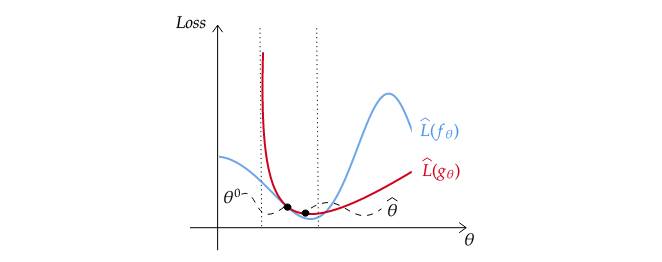
\includegraphics[scale=0.5]{figures/ntk_global_min.png}
    \caption{Here, $\hat{L}(g_{\theta})$ and $\hat{L}(f_{\theta})$ are both plotted. At $\hat{\theta}$, we have reached the approximate global minimum where $\hat{L}(g_{\hat{\theta}}) \approx 0$, in turn implying also that $\hat{L}(f_{\hat{\theta}}) \approx 0$.}
    \label{lec13:fig:ntkglobalmin}
\end{figure}

Note (1), (2), and (3) can all be true in various settings. In particular, to attain all three, we will require: 
\begin{enumerate}[label=\alph*]
    \item[(a)] Overparametrization and/or a particular scaling of the initialized $\theta^0$. 
    \item[(b)] Small (or even zero) stochasticity, so $\theta$ never leaves $B(\theta^0)$. This condition is guaranteed by a small learning rate or full-batch gradient descent. 
\end{enumerate} 
Despite the limitations of the requirements of (a) and (b), the existence of such a region is still surprising. Given the loss landscape which could potentially be highly non-convex, it is striking to find a neighborhood where the loss function is convex (e.g. quadratic) with a global minimum. This suggests there is some flexibility in the loss landscape.  

To begin our formal discussion, we  start by providing tools for proving (1) and (2). Let 
\begin{align}
    \phi^{(i)} = \phi(x\sp{i}) = \nabla_\theta f_{\theta^0}( x\sp{i}) \in \R^p
\end{align}
and 
\begin{align}
    \Phi = \begin{bmatrix} {\phi\sp{1}}^\top \\ \vdots \\ {\phi\sp{n}}^\top \end{bmatrix} \in \R^{n \times p}
\end{align}
where $p$ is the number of parameters. Taking the quadratic loss, we have
\begin{align}
    \hat{L}(g_\theta) = \frac{1}{n}\sum_{i=1}^n \left( y\sp{i} - \phi\l(x\sp{i} \r)^\top \Delta \theta \right)^2 = \frac{1}{n} \norm{\vec{y} - \Phi \cdot \Delta \theta}_2^2
\end{align} 
where $\vec{y} = \l[ y\sp{1}, \cdots, y\sp{n} \r]^\top \in \R^n$. Note that this looks a lot like linear regression, where $\Phi$ and $\Delta \theta$ are the analogues of the design matrix and parameter, respectively. We further assume that $y^{(i)} = O(1)$ and $\norm{y}_2 = O(\sqrt{n})$. Now, we can prove a lemma that addresses the second of the three conditions we described above, i.e. that it is sufficient to optimize in some small ball around $\theta^0$.

\begin{lemma}[for (2)] \label{lec13:lma:nearest_minimum}
    Suppose we are in the setting where $p \geq n$, $\textup{rank}(\Phi) = n$, and $\sigma_{\min}(\Phi) = \sigma > 0$. Then, letting $\Delta \hat{\theta}$ denote the minimum norm solution, i.e. the nearest global minimum, of $\vec{y} = \Phi \Delta \theta$, we have 
    \begin{align} 
        \norm{\Delta \hat{\theta}}_2 \leq O(\sqrt{n} / \sigma)
    \end{align} 
\end{lemma}
\begin{remark} \label{lec13:rmk:intuitiononlemma} 
    The meaning of the bound on $\Delta \hat{\theta}$ becomes clear if we consider the ball given by 
    \begin{align}
        B_{\theta^0} = \{ \theta = \theta^0 + \Delta \theta: \norm{\Delta \theta}_2 \leq O(\sqrt{n}/\sigma )\}.
    \end{align} 
    In particular, notice that $B_{\theta^0}$ contains a global minimum, so this lemma characterizes how large the ball must be to contain a global minimum. 
    \end{remark} 
\begin{remark}
	We also note that the condition $\textup{rank}(\Phi) = n$ and $\sigma > 0$ can be thought of as a ``finite-sample expressivity'' condition, saying that the features $\Phi$ are expressive enough so that there exists a linear model on top of these features that perfectly fit the data. The condition $\textup{rank}(\Phi) = n$ requires $p \ge n$---so we need some amount of over-parameterization to apply these analysis. 
\end{remark}
\begin{proof}
    Letting $\Phi^+$ denote the Moore-Penrose pseudoinverse of $\Phi$, note that $\Delta \hat{\theta} = \Phi^+ \boldsymbol{y}$, and $\norm{\Phi^+} _{\text{op}} = \frac{1}{\sigma_{\min} (\Phi)} = \frac{1}{\sigma}$.  A simple argument shows 
    \begin{align}
        \norm{\Delta \hat{\theta}}_2 &\leq \norm{\Phi^+}_{\text{op}} \cdot \norm{\vec{y}}_2 \\
        &\leq O\left( \frac{1}{\sigma}\cdot \sqrt{n} \right),
    \end{align} 
    where the last inequality follows from the assumption that $\norm{\vec{y}}_2 \leq O(\sqrt{n})$. 
\end{proof}
Next, we prove a lemma that addresses the first of the three steps we described above.
\begin{lemma}[for (1)] 
    \label{lec13:lma:accurate_approximation}
    Suppose $\nabla_\theta f_\theta(x)$ is $\beta$-Lipschitz in $\theta$, i.e. for every $x$, and $\theta, \theta'$, we have 
    \begin{align}
        \norm{\nabla_\theta f_{\theta} (x) - \nabla_{\theta} f_{\theta'}(x)}_2 \leq \beta \cdot \norm{ \theta - \theta'}_2.
    \end{align} 
    Then, 
    \begin{align} 
        \left| f_\theta(x) - g_\theta(x) \right| \leq O \left( \beta \norm{\Delta \theta}_2^2 \right).
    \end{align}  
    If we further restrict our choice of $\theta$ using $B_{\theta^0}$ as defined in Remark~\ref{lec13:rmk:intuitiononlemma}, we obtain that
    \begin{align} 
        | f_\theta(x) - g_\theta(x) | \leq O \left( \frac{\beta n }{\sigma^2 }\right), \quad \forall \theta \in B_{\theta^0}. \label{lec13:eqn:lemma1bound} 
    \end{align} 
\end{lemma}
\begin{proof}
    The proof comes from the following fact:  if $h(\theta)$ is such that $\nabla h(\theta)$ is $\beta$-Lipschitz (which if differentiable is equivalent to $\norm{\nabla^2 h(\theta)}_{\text{op}} \leq \beta$), then
    \begin{align}
        \bigg| \underbrace{h(\theta)}_{f_\theta(x)}  \underbrace{-h(\theta^0) - \inprod{\nabla h(\theta^0), \theta-\theta^0}}_{-g_\theta(x)}\bigg| \leq O\left( \beta \norm{\theta-\theta^0}_2^2 \right).
    \end{align} 
    \tnotelong{add a lemma in the toolbox section about this}
    As shown above, the proof is as simple as plugging in $f_\theta(x) = h(\theta)$ and $g_\theta(x)=h(\theta^0) + \inprod{\nabla h(\theta^0), \Delta \theta}$. 
\end{proof}

\begin{remark}
The lemma above bounds the approximation error. Intuitively, as you move farther away from $\theta^0$, the Taylor approximation gets worse; the approximation error is bounded above by a second order $\Delta \theta$ term.
\end{remark}

\begin{remark}
Note that if $f_\theta$ involves a $\text{relu}$ function, then $\nabla f_\theta$ is not continuous everywhere. This requires a technical fix outside the scope of our discussion.\footnote{A $\text{relu}$ function is continuous almost everywhere, so we can make some minor fixes and still use some modified notion of Lipschitzness to derive an upper bound.} \tnote{Tengyu will add a reference here}
\end{remark}

\subsec{Two examples of the NTK regime} \label{sec:ntk:two_examples}
By \eqref{lec13:eqn:lemma1bound}, we have now established a bound on our approximation error, but we have yet to analyze how good it is, as $\beta n /\sigma^2$ is neither obviously either big nor small. An important fact to notice is that $\beta/\sigma^2$ is not scaling invariant, so we can play with the scaling in order to drive this term to $0$. In particular, there are two notable cases (with specific parameterization, initialization, etc) where $\beta/\sigma^2 \to 0$. In the literature, such situation is often referred to as the NTK regime or the lazy training regime~\cite{chizat2018note}. 
\begin{enumerate}
    \item  \textbf{Reparameterize with a scalar} \cite{chizat2018note}. Let $f_\theta(x) = \alpha \cdot \bar{f}_\theta(x)$ where $\bar{f}_\theta(x)$ is an arbitrary neural net with fixed width and depth. We only vary $\alpha$, i.e. the scaling, and we see how the crucial quantity $\beta/\sigma^2$ changes accordingly. Fix an initial $\theta^0$, and let 
    \begin{align}
        \bar{\sigma} = \sigma_{\min}\left( \begin{bmatrix}  \nabla_\theta \bar{f}_{\theta^0} \big( x^{(1)} \big)^\top \\ \vdots \\ \nabla_\theta \bar{f}_{\theta^0} \big(x^{(n)} \big)^\top \end{bmatrix}\right).
    \end{align} 
    Furthermore, let $\bar{\beta}$ be the Lipschitz parameter of $\nabla_\theta \bar{f}_\theta(x)$ in $\theta$. A simple chain-rule gradient argument shows that scaling $\bar{f}_{\theta}$ by $\alpha$ also scales $\sigma$ and $\beta$ accordingly, i.e. $\sigma = \alpha \bar{\sigma}$, and $\beta = \alpha \bar{\beta}$. Some straightforward algebra yields 
    \begin{align} 
        \frac{\beta}{\sigma^2}= \frac{\bar{\beta}}{\bar{\sigma}^2} \cdot \frac{1}{\alpha} \to 0 \quad \text{as} \quad \alpha \to \infty.
    \end{align}
    Once $\alpha$ becomes big enough, then by Lemma~\ref{lec13:lma:accurate_approximation}, the approximation $|f_\theta(x) - g_\theta(x)| \leq O\left( \beta n / \sigma^2 \right)$ becomes very good. 
    
\begin{remark} A priori, such a phenomenon may appear to be too good to be true. To understand it better, we first note that this re-parameterizaton does not change the scale of the loss, but rather change the shape of the loss function. Intuitively, as $\alpha$ becomes larger, the function $f_\theta$ becomes sharper and more non-smooth (leading to higher approximation error). However, on the other hand, we note that we only need to travel a little bit away from $\theta^0$ to find a global minimum given that there is a global minimum within radius $O(\sqrt{n}/\sigma)$. It turns out that the radius needed shrinks faster than the smoothness grows. 
    
    To visualize this effect, we can consider the following example with only 1 data point with 1-dimensional input $(x,y) = (1,1)$ and the quadratic model $\bar{f}_\theta(x) = x(\theta + \beta \theta^2) = \theta + \beta \theta^2$. Using the squared loss, we have 
    \begin{align}
    \hatL(\bar{f}_\theta) = (1- (\theta + \beta \theta^2))^2 
    \end{align}
    Let $\theta^0 = 0$. Taylor expanding at $\theta^0$ gives the linear approximation $\bar{g}_\theta(x) = \theta x$ = $\theta$, and the resulting loss function that is quadratic 
    \begin{align}
    \hatL(\bar{g}_\theta) = (1- \theta)^2 
    \end{align}
	In this case,  $\nabla f_{\theta^0}(x) = 2\beta \theta x = 2\beta \theta$ is $2\beta$-Lipschitz, and $ \sigma = 1$. 
	
	Now we vary $\alpha$ and get 
    \begin{align}
\hatL(\alpha \bar{f}_\theta) = (1- \alpha(\theta + \beta \theta^2))^2 
\end{align}	
and 
\begin{align}
\hatL(\alpha\bar{g}_\theta) = (1- \alpha\theta)^2 
\end{align}
Note that the minimizer of $	\hatL(\alpha\bar{g}_\theta) $ is $1/\alpha$, which is closer to $\theta^0$ as $\alpha\rightarrow \infty$. We zoom into the region $[0, 1/\alpha]$ and find out the difference between $\alpha \bar{f}_\theta$ and $\alpha \bar{g}_\theta$ is $\alpha \beta\theta^2 \le  \beta/\alpha$, which is much smaller than the value of $\alpha \bar{g}_\theta \approx O(1)$. 

We visualize the these functions in Figure~\ref{fig:ntk-1d}. We observe that $\hatL(\alpha\bar{g}_\theta) $ becomes a better approximation of $\hatL(\alpha\bar{f}_\theta)$ in the region $[0,1/\alpha]$ as $\alpha \rightarrow \infty$ (though $\hatL(\alpha\bar{g}_\theta)$ is a worse approximation of $\hatL(\alpha\bar{f}_\theta)$ globally.)


\begin{figure}[t]
	\centering
	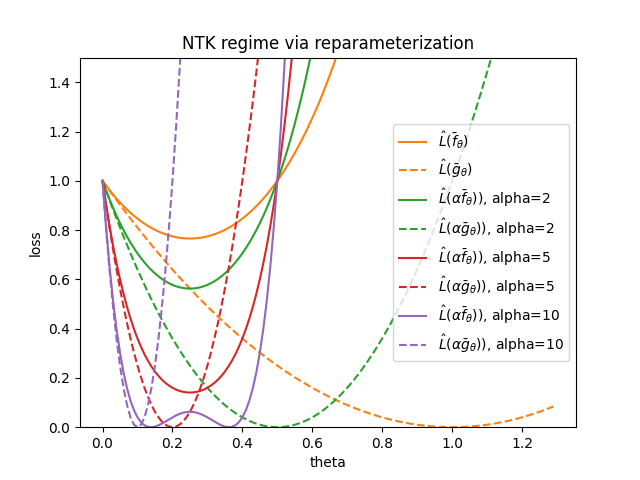
\includegraphics[width = 0.6\textwidth]{figures/ntk-1d.png}
	\caption{\label{fig:ntk-1d} The approximation $\hatL(\alpha\bar{g}_\theta) $ becomes a better approximation of $\hatL(\alpha\bar{f}_\theta)$ in the region $[0,1/\alpha]$ as $\alpha \rightarrow \infty$ (though $\hatL(\alpha\bar{g}_\theta)$ is a worse approximation of $\hatL(\alpha\bar{f}_\theta)$ globally).}
\end{figure}
	%The minimum norm solution with $\alpha g_\theta$ is
%    \[
%    \argmin{\theta} (1-\alpha  \theta)^2 = 1/\alpha.
%    \]
%    Now, for $\alpha\geq 1$ we compute
%    \[
%    D(\alpha) = \sup_{\theta\in [0,1/\alpha ]} |\alpha f_\theta(1) - \alpha g_\theta(1)|. 
%    \]
%    We will plot $D(\alpha)$ as well as $\hat L(\alpha f_\theta(1))$ and $\hat L(\alpha g_\theta(1))$ for $\alpha = 1,2,4$. In the following plots, we use $\beta = 2$. 
%   
\end{remark}
    \item \textbf{Overparametrization (with specific initialization)}. Early papers on the NTK take this approach (e.g., ~\cite{li2018learning,du2019gradient}). Consider a  two-layer network with $m$ neurons. 
    \begin{align}
        \hat{y} = \frac{1}{\sqrt{m}} \sum_{i=1}^m a_i \sigma(w_i^\top x )
    \end{align} 
    The scaling $1/\sqrt{m}$ is to ensure that a random initialization with constant scale will have output on the right order, as we see momentarily. We make the following assumptions regarding the network and its inputs.
    \begin{align}
        W &= \begin{bmatrix} w_1^\top \\ \vdots \\ w_m^\top \end{bmatrix} \in \R^{m \times d} \\
        \sigma &\text{ is $1$-Lipschitz and twice-differentiable} \\
        a_i &\sim \{\pm 1\} \quad &\text{(not optimized)} \\
        w_i^0 &\sim \cN(0, I_d) \\
        \norm{x}_2 &= \Theta(1) \\
        \theta &= \text{vec}(W) \in \R^{dm} \quad &\text{(vectorized $W$)}
    \end{align} 
    We will assume $m \to \infty$ polynomially in $n$ and $d$. In particular, for fixed $n,d$, we have $m = \textsf{poly}(n,d)$.
    
    Why do we use the $1/\sqrt{m}$ scaling? Note that $\sigma\big({w_i^0}^\top x\big) \approx 1$ because $\norm{x}_2 = \Theta(1)$ and $w_i^0$ is drawn from a spherical Gaussian. Thus, as some $a_i$ are positive and others are negative, $\left|\sum_{i=1}^m a_i \sigma \big({w_i^0}^\top x\big) \right| = \Theta \left( \sqrt{m} \right)$, and finally $f_{\theta^0} (x) = \Theta(1)$. 
    
    Now we analyze $\sigma$ and $\beta$. We let
    \begin{align}
        \sigma = \sigma_{\min} (\Phi) = \sqrt{\sigma_{\min} \left( \Phi \Phi^\top \right)}
    \end{align}
    where 
    \begin{align}
        \left( \Phi \Phi^\top \right)_{ij} = \inprod{\nabla_\theta f_{\theta^0} \big(x^{(i)} \big) , \nabla_\theta f_{\theta^0} \big(x^{(j)} \big)} \label{lec13:eqn:phifeature} 
    \end{align} 
    Note that the gradient with respect to $w_i$ is given by 
    \begin{align}  
        \frac{\partial f_\theta(x) }{\partial w_i} = \frac{1}{\sqrt{m}} \sigma'(w_i^\top x ) \cdot x 
    \end{align} 
    Now observe that
    \begin{align}
        \norm{\nabla f_\theta(x)}_2^2 & = \frac{1}{m}\sum_{i=1}^m \norm{\sigma'\big({w_i}^\top x \big) \cdot x }_2^2 \\ 
        & = \frac{1}{m}\norm{x}_2^2 \cdot \sum_{i=1}^m \left( \sigma' \big({w_i}^\top x \big) \right)^2 \\ 
        &\to \Exp_{w \sim \cN(0,I_d)} \left[ \sigma' \big( w^\top x \big)^2 \right] \cdot \norm{x}_2^2 \quad \text{as} \quad m\to\infty \\ 
        &= O(1) &\text{(not depending on $m$)}
    \end{align} 
    where the penultimate line follows from the law of large numbers, as $\frac{1}{m} \sum_{i=1}^m \left( \sigma'(w_i^\top x ) \right)^2$ can be interpreted as a mean. 
    
    Note that the scale of $\norm{\nabla_\theta f_{\theta^0} (x)}_2$ does not depend on $m$, so the inner product in \eqref{lec13:eqn:phifeature} also does not depend on $m$ either. As above, we can show 
    \begin{align} 
        \inprod{\nabla_\theta f_{\theta^0} (x), \nabla_\theta f_{\theta^0} (x')} & = \frac{1}{m}\inprod{ x,x'} \sum_{i=1}^m \sigma'(w^\top x) \sigma'(w^\top x')  \\ 
        & \to \Exp_{w \sim \cN(0,I_d)} \left[ \sigma'(w^\top x) \sigma'(w^\top x') \right] \inprod{ x, x'} \label{lec13:eqn:kernelcalc} 
    \end{align}
    
    \eqref{lec13:eqn:kernelcalc} implies that as $m \to \infty$, $\Phi \Phi^\top$ converges to a constant matrix denoted by 
    \begin{align}
        K^\infty = \lim_{m \to \infty} \Phi\Phi^\top 
    \end{align}
    This is precisely the NTK with $m=\infty$.  Though we omit the proof of this claim, it can be shown that $K^\infty$ is full rank. Then, let \begin{align}
        \sigma_{\min} \triangleq \sigma_{\min} (K^\infty) > 0.
    \end{align}
    We can show that 
    \begin{align}
        \sigma = \sigma_{\min} \left( \Phi \Phi^\top \right) > \frac{1}{2}\sigma_{\min} 
    \end{align} 
    Intuitively, $\Phi \Phi^\top \to K^\infty$, so the spectrum of the matrix should also converge. Thus, in some sense, we have shown that $\sigma$ is constant in the limit. 
    
    Now what about $\beta$? If we can show $\beta \to 0$ as $m \to \infty$, we are done. We begin by analyzing this key expression:  
    \begin{align}
        \nabla_\theta f_\theta(x) - \nabla_\theta f_{\theta'} (x) = \left[ \frac{1}{\sqrt{m}} \left( \sigma' \big( w_i^\top x \big) - \sigma' \big({w_i'}^\top x \big) \right) \cdot x \right]_{i=1}^m \label{lec13:eqn:lipschitzmatrix}
    \end{align}
    Note that \eqref{lec13:eqn:lipschitzmatrix} above consists of matrices, as $\theta$ is a vectorized matrix. Then,
    \begin{align}
        \norm{\nabla_\theta f_\theta(x) - \nabla_\theta f_{\theta'}(x)}_2^2 & = \frac{1}{m}\sum_{i=1}^m \norm{x}_2^2 \left( \sigma' \big(w_i^\top x \big) - \sigma' \big({w_i}'^\top x \big) \right)^2  \\ 
        & \leq O \left( \frac{1}{m}\sum_{i=1}^m \norm{ x}_2^2 \big( w_i^\top x - {w_i'}^\top x \big)^2 \right) \\ 
        & =  O \left( \frac{1}{m}\sum_{i=1}^m \norm{ w_i - w_i'}_2^2 \right) \\ 
        & = O \left(\frac{1}{m} \norm{ \theta - \theta' }_2^2 \right)
    \end{align} 
    The first line follows from the fact that $\frac{1}{\sqrt{m}} \left( \sigma' \big( w_i^\top x \big) - \sigma' \big({w_i'}^\top x \big) \right)$ is a scalar. The second line uses the assumption that $\sigma'$ is $O(1)$-Lipschitz. The third line uses Cauchy-Schwarz and the fact that $\norm{x}_2^2 \approx 1$. Taking the square root, we have that
    \begin{align} 
        \norm{\nabla_\theta f_\theta(x) - \nabla_\theta f_{\theta'}(x)}_2 \lesssim \frac{1}{\sqrt{m} } \norm{ \theta -\theta' }_2
    \end{align} 
    Thus, the Lipschitz parameter is $\beta = O(1/\sqrt{m})$. Thus, our key quantity $\beta/\sigma^2$ goes to $0$ as $m$ grows. Namely,
    \begin{align} 
        \frac{\beta}{\sigma^2} \approx \frac{1}{\sqrt{m} }\cdot \frac{1}{\sigma_{\min}^2} \to 0 \quad \text{as} \quad m\to\infty.
    \end{align} 
    Recall here that $\sigma_{\min}$ does not depend on $m$. Concretely, this result tells us that our function becomes more smooth (the gradient has a smaller Lipschitz constant) as we add more neurons. 
\end{enumerate}

\subsec{Optimizing $\hat{L}(g_\theta)$ vs. $\hat{L}(f_\theta)$}
We now discuss how to establish the last of the three conditions under which we claimed a Taylor approximation is reasonable. We need to show that  optimizing $\hat{L} (f_\theta)$ is similar to optimizing $\hat{L}(g_\theta)$. To do so, we require two steps:
\begin{enumerate}[label=\alph*]
    \item[(A)] Analyze optimization of $\hat{L}(g_\theta)$.
    \item[(B)] Analyze optimization of $\hat{L}(f_\theta)$ by re-using or modifying the proofs in (A).
\end{enumerate}
There are two approaches in the literature for (A), which implies that there exist two approaches for (B) as well. 
\begin{enumerate}
    \item[(i)] We leverage the strong convexity of $\hat{L} (g_\theta)$, and then show an exponential convergence rate.\footnote{Recall that a differentiable function $f$ is $\mu$-strongly convex if 
    \begin{align} 
        f(y) \geq f(x) + \nabla f(x)^\top (y-x) + \frac{\mu}{2} \norm{y-x}_2^2
    \end{align} for some $\mu>0$ and all $x,y$.} 
    \item[(ii)] Instead of strong convexity, we rely on the smoothness of $f_\theta$ (i.e. bounded second derivative). 
\end{enumerate}
We will only discuss the first of these two methods in the sequel.

\begin{remark} In both either approach (i) or (ii), we will implicitly or explicitly use the following simple fact. 
Suppose at any $\theta^t$, we take the Taylor expansion of $f_\theta$ at $\theta^t$:
\begin{align} 
    g_\theta^t(x) = f_{\theta^t} (x) + \inprod{ \nabla f_{\theta^t} (x),\theta-\theta^t } 
\end{align} 
Consider the gradient we are interested in taking: $\nabla \hat{L} ( f_{\theta^t})$. Notice that: \begin{align} 
    \nabla \hat{L} ( f_{\theta^t}) = \nabla \hat{L} ( g_{\theta^t}^t)
\end{align} 
This is really saying that $f_\theta$ and $g_\theta^t$ agree up to first-order at $\theta^t$. This implies that $L(f_\theta)$ and $L(g_\theta^t)$ also agree to first-order at $\theta^t$. This also means that $T$ steps of gradient descent on $\hat{L}(f_\theta)$ is the same as performing online gradient descent\footnote{Online gradient descent is the algorithm that takes one gradient descent step upon receiving a new objective function. See Chapter~\ref{chap:OL} for more discussions about online learning.} on a sequence of changing objectives $L(g_\theta^0), \ldots, L(g_\theta^T)$, and this online learning perspective is useful in the approach (ii). 
\end{remark} 

We will now show that under the strong convexity regime, optimizing a neural network $f_\theta$ is equivalent to optimizing a linear model $g_\theta$. We will also observe that this regime is not particularly practically relevant, but this analysis is nevertheless of interest to us for two reasons. First, the approach used in the subsequent exposition is of technical interest and second, it remains quite interesting that optimizing $f_\theta$ and optimization $g_\theta$ yields the same results under \emph{any} regime. 

\subsubsec{Optimizing $g_\theta$}
We relate the optimization of $g_\theta$ to performing linear regression. Recall that we can think of $\nabla f_{\theta^0}(x)$ as a feature map. Then, the problem of choosing $\Delta \theta$ to get $g_\theta(x)$ to be close to $\vec{y}$ is a linear regression. In particular, we use gradient descent to minimize
\al{
\norm{\vec{y} - \Phi\Delta \theta}_2^2,
}
where 
\al{
\Phi =
\begin{bmatrix}
\nabla f_{\theta^0}(x^{(1)})^\top \\
\vdots \\
\nabla f_{\theta^0}(x^{(n)})^\top
\end{bmatrix}
\in \R^{n \times p}. 
\quad \quad \vec{y} = \begin{bmatrix} y\sp{1} \\ \vdots\\ y\sp{n} \end{bmatrix} \in \R^n
}
For learning rate $\eta$, the gradient descent update rule is 
\al{
{\Delta \theta}^{t+1} = \Delta \theta^{t} - \eta \Phi^\top (\Phi \Delta \theta^t - \vec{y}). \label{lec14:eqn:update-rule}
}
This analysis considers changes in the output space. Define $\hat{y}^t = \Phi \Delta \theta^t$. Then, we're interested in changes in 
\al{
\hat{y}^{t+1} - \vec{y} &= \Phi \Delta \theta^{t+1} - \vec{y}\\
&= \Phi \left( \Delta \theta^{t} - \eta \Phi^\top (\Phi \Delta \theta^t - \vec{y})\right) - \vec{y} &\text{(by \eqref{lec14:eqn:update-rule})}\\
&= \left( \Phi - \eta \Phi \Phi^\top \Phi\right)\Delta \theta^t - (I - \eta \Phi \Phi^\top)\vec{y}\\
&= (I - \eta \Phi \Phi^\top )\Phi \Delta \theta^t - (I - \eta \Phi \Phi^\top )\vec{y}\\
&= (I - \eta \Phi \Phi^\top) (\Phi \Delta \theta^t - \vec{y})\\
&= (I - \eta \Phi \Phi^\top)(\hat{y}^t - \vec{y}). \label{lec14:eqn:g_decomp}
}
From this decomposition, we see that the residuals, $\hat{y}^t - \vec{y}$, are monotonically shrinking since $\eta \Phi \Phi^\top$, i.e. the term we are subtracting from $I$ in \eqref{lec14:eqn:g_decomp}, is positive semidefinite. Next, we quantify how quickly we are shrinking the residuals. Define 
\begin{align}
    \tau^2 &= \sigma_{\text{max}}(\Phi \Phi^\top) \\
    \sigma &= \sigma_\text{min}(\Phi) = \sqrt{\sigma_\text{min}(\Phi\Phi^\top)}. \label{lec14:eqn:sigma_def}
\end{align}
Then, we claim that when $\eta \leq \frac{1}{\tau^2}$,
\al{
\norm{I - \eta \Phi \Phi^\top }_{\text{op}} \leq 1-\eta \sigma^2. \label{lec14:eqn:g_decomp_op}
}
Why? Let the eigenvalues of $\Phi \Phi^\top$ be (in descending order) $\tau_1^2, \dots , \tau_n^2$. By definition, $\tau_1^2 = \tau^2$ and $\tau_n^2 = \sigma^2$. Now, given the singular value decomposition, $\Phi = U\Sigma V^\top$, we obtain the eigendecomposition: 
\al{
I - \eta \Phi \Phi^\top &= I - \eta U \Sigma^2 U^\top \\
&= U U^\top - \eta U \Sigma^2 U^\top \\ 
&= U(I - \eta \Sigma^2)U^\top \label{lec14:eqn:g_coeff_eigendecomposition}.
}
\eqref{lec14:eqn:g_coeff_eigendecomposition} is the eigendecomposition of $I - \eta \Phi \Phi^\top$, so $I - \eta \Phi \Phi^\top$ has eigenvalues $1 - \eta \tau_1^2, \dots, 1 - \eta \tau_n^2$.
\tnote{maybe explain why this is the case by taking an SVD? see screenshot} Note that assuming $\eta \leq \frac{1}{\tau^2}$ ensures that all eigenvalues of $I - \eta \Phi \Phi^\top$ are non-negative. Thus,
\al{
\norm{I - \eta \Phi \Phi^\top}_\text{op} &\leq \max_j |1-\eta \tau_j^2|\\
&= 1 - \eta \tau_n^2 \label{lec14:eqn:eigenvalue_bound}\\
&= 1 - \eta \sigma^2,
}
where the non-negativity of $1 - \eta \tau_j^2$ for all $j$ implies \eqref{lec14:eqn:eigenvalue_bound}.

Using this result, we obtain our desired result. Namely, assuming $\eta \leq \frac{1}{\tau^2}$,
\al{
\norm{\hat{y}^{t+1} - \vec{y}}_2 &= \norm{I - \eta \Phi \Phi^\top }_\text{op} \cdot \norm{\hat{y}^t - \vec{y}}_2 \\
&\leq (1-\eta\sigma^2)\norm{\hat{y}^t - \vec{y}}_2 \\
&\leq (1 - \eta \sigma^2 )^{t+1}\norm{\hat{y}^0 - \vec{y}}_2.
}
This yields the desired exponential decay in the error. Thus, after $T = O \l( \frac{\log 1/\epsilon}{\eta \sigma^2}\r)$ iterations, 
\al{
\norm{ \hat{y}^T - \vec{y} }_2 \leq \epsilon \norm{\hat{y}^0 - \vec{y}}_2. \label{lec14:eqn:g_exponential_decay}
}

\subsubsec{Optimizing $f_\theta$}
We now transition to an analysis of the optimization of $f_{\theta}$. Our key result is Theorem \ref{lec14:thm:optimization_f}. If we compare it against what we have in \eqref{lec14:eqn:g_exponential_decay}, we see the claimed similarity between $f_\theta$ and $g_\theta$ in error decay under optimization. 

\begin{theorem}
There exists a constant $c_0 \in (0, 1)$ such that for $\frac{\beta}{\sigma^2} \leq \frac{c_0}{n}$ and sufficiently small $\eta$ (which could depend on $\beta, \sigma$, or $p$), $\hat{L}\l(f_{\theta^T}\r) \leq \epsilon$ after $T = O \l(\frac{\log 1/\epsilon}{\eta\sigma^2}\r)$ steps. \label{lec14:thm:optimization_f} 
\end{theorem}

\begin{proof}

(This is actually a proof sketch that elides a few technical details for the sake of a simpler exposition.) Our approach is to follow the preceding analysis of $g_\theta$, making changes where necessary.

Let  
\al{
\Phi^t =
\begin{bmatrix}
\nabla f_{\theta^t}(x^{(1)})^\top \\
\vdots \\
\nabla f_{\theta^t}(x^{(n)})^\top
\end{bmatrix}
\in \R^{n \times p}.
}
To obtain our gradient descent update rule, we find, using the chain rule,
\begin{align}
    \nabla \hat{L}\l(f_{\theta^t}\r) &=  \sum_{i=1}^n\l(f_{\theta^t}\l(x^{(i)}\r) - y^{(i)}\r)\nabla f_{\theta^t}\l(x^{(i)}\r) \\ 
    &=  \sum_{i=1}^n\l(\hat{y}^{(i), t} - y^{(i)}\r)\nabla f_{\theta^t}\l(x^{(i)}\r) \\
    &= (\Phi^t)^\top\l(\hat{y}^t - \vec{y}\r).
\end{align}
This results in the policy
\begin{align}
    \theta^{t+1} &= \theta^t - \eta \nabla \hat{L}\l(f_{\theta^t}\r) \\
    &= \theta^t - \eta (\Phi^t)^\top\l(\hat{y}^t - \vec{y}\r) \\ 
    &= \theta^t - \eta b^t,
\end{align}
where we have let $b^t = (\Phi^t)^\top\l(\hat{y}^t - \vec{y}\r)$. Following our treatment of $g_\theta$, we want to express $\hat{y}^{t+1}$ as a function of $\hat{y}^{t}$. The challenge now is that $f$ is nonlinear. To deal with this, we Taylor expand $f_\theta$ at $\theta_t$:

\begin{align}
   f_{\theta^{t+1}}(x^{(i)}) &= f_{\theta^{t}}(x^{(i)}) + \l<\nabla f_{\theta^t}(x^{(i)}), \theta^{t+1} - \theta^t \r> + \text{high order terms} \\
   &= f_{\theta^{t }}(x^{(i)}) + \l<\nabla f_{\theta^t}(x^{(i)}), -\eta b^t \r> + O\l(\norm{\theta^{t+1} - \theta^t}_2^2\r). \label{lec14:eqn:f_taylor_expansion}
 \end{align}
Since $O\l(\norm{\theta^{t+1} - \theta^t}_2^2\r)$ is $O\l(\eta^2\r)$, we can ignore this term as $\eta \rightarrow 0$. Vectorizing \eqref{lec14:eqn:f_taylor_expansion} without $O\l(\norm{\theta^{t+1} - \theta^t}_2^2\r)$,
\begin{align}
    \hat{y}^{t+1} &= \hat{y}^t - \eta \Phi^t b^t \\
    &= \hat{y}^t + \eta \Phi^t\l(\Phi^t\r)^\top(\vec{y} - \hat{y}^t).
\end{align}
Subtracting $\vec{y}$ and re-arranging,
\begin{align}
    \hat{y}^{t+1} - \vec{y} &= \hat{y}^t - \vec{y} + \eta \Phi^t\l(\Phi^t\r)^\top(\vec{y} - \hat{y}^t) \\ 
    &= \l(I - \eta \Phi^t\l(\Phi^t\r)^\top\r)\l(\hat{y}^t - \vec{y}\r). \label{lec14:eqn:f_decomposition}
\end{align}
Comparing \eqref{lec14:eqn:f_decomposition} with \eqref{lec14:eqn:g_decomp}, we see one difference: in \eqref{lec14:eqn:f_decomposition}, our convergence depends on $\eta \Phi^t\l(\Phi^t\r)^\top$, which is a matrix that changes as we iterate, whereas in \eqref{lec14:eqn:g_decomp}, convergence is controlled by a matrix that is fixed as we iterate. 

To understand the convergence implications of \eqref{lec14:eqn:f_decomposition}, we examine the eigenvalues of \linebreak $I - \eta \Phi^t \l(\Phi^t\r)^\top$. For now, suppose $\norm{\theta^t - \theta^0}_2 \leq \sigma/(4\sqrt{n}\beta)$ at time $t$. This implies that $\norm{\Phi^t - \Phi}_F \leq \frac{\sigma}{4}$ by the Lipschitzness of $\nabla f_\theta(x)$ in $\theta$. Here with slight abuse of notations we 
Then, we claim that 
\begin{align}
    \sigma_{\text{min}}(\Phi^t) \geq 3\sigma/4. \label{lec14:eqn:phi_t_eigenvalue_bound}
\end{align}
Why does \eqref{lec14:eqn:phi_t_eigenvalue_bound} hold? Observe that
\begin{align}
    \sigma_\text{min}(\Phi^t) &= \underset{\norm{x}_2=1}{\text{min}} x^\top \Phi^tx \\
   &\geq \underset{\norm{x}_2=1}{\text{min}} x^\top (\Phi^t - \Phi)x + \underset{\norm{x}_2=1}{\text{min}}  x^\top \Phi x. \label{lec14:eqn:eigenbound_phi_t}
\end{align}
We can lower bound the first term of \eqref{lec14:eqn:eigenbound_phi_t} as follows:
\begin{align}
    x^\top (\Phi^t - \Phi)x &\geq -|\l<x, (\Phi^t - \Phi)x\r>| \\
    &\geq -\norm{x}_2 \norm{(\Phi^t - \Phi)x}_2 &\text{(Cauchy-Schwarz)}\\ 
    &\geq -\norm{\Phi^t - \Phi}_2 &\text{($\norm{x}_2 = 1$)}\\ 
    &\geq -\sigma/4 &\text{(Lipschitzness of $\Phi$)}. \label{lec14:eqn:termone_eigenbound}
\end{align}
Next, we note that the second term of \eqref{lec14:eqn:eigenbound_phi_t} is lower bounded by $\sigma$ by simplifying and applying the definition of $\sigma$ given in \eqref{lec14:eqn:sigma_def}. Combining this observation with \eqref{lec14:eqn:termone_eigenbound}, we conclude that \eqref{lec14:eqn:phi_t_eigenvalue_bound} must hold.

Applying this lower bound on the eigenvalues of $\Phi^t$, we can use the same argument we used to establish \eqref{lec14:eqn:g_decomp_op} to conclude that
\begin{align}
    \norm{I - \eta \Phi^t \l(\Phi^t\r)^\top}_{\text{op}} \leq 1 - 3\eta \sigma/4 \label{lec14:eqn:op_norm_bound},
\end{align}
and 
\begin{align}
    \norm{\hat{y}^{t+1} - \vec{y}}_{2} \leq \l(1 - 3\eta \sigma/4\r)^{t+1} \norm{\hat{y}^{0} - \vec{y}}_{2}.
\end{align}
So, as desired, we see exponential decay in the error at each iteration and after $T = O \l( \frac{\log 1/\epsilon}{n\sigma^2}\r)$ iterations,
\al{
\hat{L}(f_{\theta^T}) \leq \epsilon.
}

To complete our proof, observe that this argument is predicated upon the assumption that $\norm{\theta^t - \theta^0}_2 \leq \sigma/(4\sqrt{n}\beta)$. This assumption is reasonable, however, given what we have already proven. Recall that in Lemma~\ref{lec13:lma:nearest_minimum}, we proved that 
\begin{align}
    \norm{\Delta \hat{\theta}}_2 = \norm{\hat{\theta} - \theta^{0}}_2 \lesssim \sqrt{n}/\sigma.
\end{align}
Thus, when $\beta/\sigma^2 \rightarrow 0$, eventually, $\sqrt{n}/\sigma \ll \sigma/(4\sqrt{n}\beta)$. To extend this to $\norm{\hat{\theta} - \theta^t}_2$ for arbitrary $t$, we heuristically argue that since the empirical minimizer is within $\sigma/(4\sqrt{n}\beta)$ of $\theta^0$, we would not expect to have traveled more than $\sigma/(4\sqrt{n}\beta)$ from $\theta^0$ at \emph{any} iteration. 

More formally, we claim that for all $t \in \mathbb{N}$, 
\al{
\norm{\hat{y}^t - \vec{y}}_2 \leq \cO (\sqrt{n}).  \label{lec14:eqn:induction}
}
We proceed via induction. For $t=0$, because each element of $\hat{y}$ is of order $1$, we know that: 
\al{
\frac{1}{\sqrt{n}} \norm{\hat{y}^0 - \vec{y}}_2 \leq O (1).
}
Now, suppose that \eqref{lec14:eqn:induction} holds for some $t$. Then, because the errors are monotonically decreasing, (cf. \eqref{lec14:eqn:f_decomposition} and \eqref{lec14:eqn:op_norm_bound}), 
\al{
\frac{1}{\sqrt{n}} \norm{\hat{y}^{t+1} - \vec{y}}_2 \leq \frac{1}{\sqrt{n}}  \norm{\hat{y}^t - \vec{y}}_2 \leq O(1).
}
Thus, \eqref{lec14:eqn:induction} holds for all $t \in \mathbb{N}$. Then, recalling that $\vec{y} = \Phi\hat{\theta}$, we obtain that
\al{
\frac{1}{\sqrt{n}} \norm{\Phi (\theta^t - \hat{\theta})}_2 &\leq O(1).
}
Then, leveraging the definition of $\sigma$ given in \eqref{lec14:eqn:sigma_def} and rearragning, we obtain (nearly) the desired result:
\al{
\norm{\theta^t - \hat{\theta}}_2 \leq \frac{1}{\sigma}\norm{\Phi (\theta^t - \hat{\theta})}_2 &\leq O(\sqrt{n}/\sigma).
}
Recall that in Lemma~\ref{lec13:lma:nearest_minimum}, we proved that 
\al{
\norm{\hat{\theta} - \theta^0}_2 \leq O(\sqrt{n}/\sigma).
}
If $\beta/\sigma^2 \ll 1/n$, we conclude that
\al{
\norm{\theta^t - \theta^0}_2 &\leq \norm{\hat{\theta} - \theta^0}_2 + \norm{\theta^t - \hat{\theta}}_2 &\text{(triangle ineq.)}\\
&\leq O\l (\frac{\sqrt{n}}{\sigma} \r ) \leq \frac{\sigma}{4\sqrt{n}\beta}. 
}
\end{proof}
\subsec{Limitations of NTK}

The NTK approach has its limitations.
\begin{itemize}
    \item Empirically, optimizing $g_\theta(x)$ as described in the theory does not work as well as state-of-the-art (or even standard) deep learning methods. For example, using the NTK approach (i.e., taking the Taylor expansion and optimizing $g_{\theta}(x)$) with a ResNet generally does not perform as well as ResNet with best-tuned hyperparameters.
    
    \item The NTK approach requires a specific initialization scheme and learning rate which may not coincide with what is commonly used in practice.
    
    \item The analysis above was for gradient descent, while stochastic gradient descent is used in practice, introducing noise in the procedure. This means that NTK with stochastic gradient descent requires a small learning rate to stay in the initialization neighborhood. Deviating from the requirements can lead to leaving the initialization neighborhood.
\end{itemize}

One possible explanation for the gap between theory and practice is because NTK effectively requires a fixed kernel, so there is no incentive to select the right features. Furthermore, the minimum $\ell_2$-norm solution is typically dense. This is similar to the difference between sparse and dense combinations of features observed in the $\ell_1$-SVM/two-layer network versus the standard kernel method SVM (or $\ell_2$-SVM) analyzed previously.

To make these ideas more concrete, consider the following example \cite{wei2020regularization}. 
\begin{example}\label{lec12:ex:sparse123}
Let $x \in \R^d$ and $y \in \{-1, 1\}$. Assume that each component of $x$ satisfies $x_i \in \{ -1, 1\}$. Define the output $y = x_1x_2$, that is, $y$ is only a function of the first two components of $x$.

This output function can be described exactly by a neural network consisting of a sparse combination of the features (4 neurons to be exact):
\begin{align}
\hat y &= \frac{1}{2} \left[ \phirelu(x_1 + x_2) + \phirelu(-x_1 - x_2)  - \phirelu(x_1 - x_2) -  \phirelu(x_2 - x_1)  \right] \\
&= \frac{1}{2}\left( |x_1 + x_2| - |x_1 - x_2| \right) \label{lec12:eqn:ex1} \\
&= x_1x_2. \label{lec12:eqn:ex2}
\end{align}
\eqref{lec12:eqn:ex1} follows from the fact that $\phirelu(t) + \phirelu(-t) = |t|$ for all $t$, while \eqref{lec12:eqn:ex2} follows from evaluating the 4 possible values of $(x_1, x_2)$. Thus, we can solve this problem exactly with a very sparse combination of features.

However, if we were to use the NTK approach (kernel method), the network's output will always involve $\sigma(w^\top x)$ where $w$ is random so it includes all components of $x$ (i.e. a dense combination of features), and cannot isolate just the relevant features $x_1$ and $x_2$. This is illustrated in the following informal theorem:
\begin{theorem}
The kernel method with NTK requires $n = \Omega(d^2)$ samples to learn Example \ref{lec12:ex:sparse123} well. In contrast, the neural network regularized by $\sum_{j = 1}^m | u_j| \| w_j\|_2$ only requires $n = O(d)$ samples.
\end{theorem}
\end{example}


